\documentclass[tikz,border=6pt]{standalone}
\usepackage{tikz}
\usetikzlibrary{positioning,arrows.meta}
\usepackage{xcolor}

\definecolor{gitopsblue}{RGB}{51,108,229}
\definecolor{manualgray}{RGB}{102,102,102}
\definecolor{metricyellow}{RGB}{251,192,45}
\definecolor{driftred}{RGB}{229,115,115}

\begin{document}
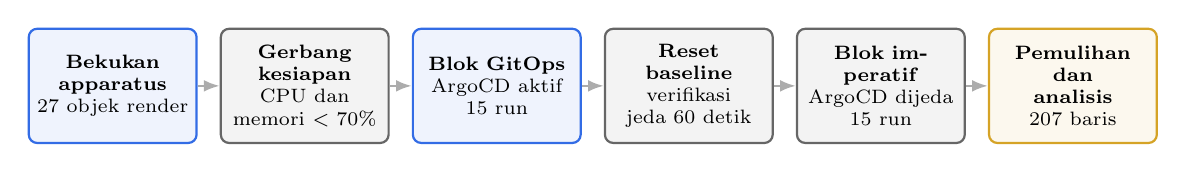
\begin{tikzpicture}[
    node distance=0.28cm,
    box/.style={rectangle, rounded corners=3pt, draw=#1, fill=#1!8,
                text width=1.92cm, minimum height=1.45cm, align=center,
                line width=0.8pt, font=\scriptsize, inner sep=3pt},
    arrow/.style={-{Latex[length=2mm]}, line width=0.9pt, draw=gray!65}
]

\node[box=gitopsblue] (freeze) {
    \textbf{Bekukan}\\\textbf{apparatus}\\27 objek render
};
\node[box=manualgray, right=of freeze] (gate) {
    \textbf{Gerbang}\\\textbf{kesiapan}\\CPU dan memori $<70\%$
};
\node[box=gitopsblue, right=of gate] (gitops) {
    \textbf{Blok GitOps}\\ArgoCD aktif\\15 run
};
\node[box=manualgray, right=of gitops] (reset) {
    \textbf{Reset baseline}\\verifikasi\\jeda 60 detik
};
\node[box=manualgray, right=of reset] (imp) {
    \textbf{Blok imperatif}\\ArgoCD dijeda\\15 run
};
\node[box=metricyellow!85!black, right=of imp] (analysis) {
    \textbf{Pemulihan dan}\\\textbf{analisis}\\207 baris
};

\draw[arrow] (freeze) -- (gate);
\draw[arrow] (gate) -- (gitops);
\draw[arrow] (gitops) -- (reset);
\draw[arrow] (reset) -- (imp);
\draw[arrow] (imp) -- (analysis);

\end{tikzpicture}
\end{document}
